\documentclass[11pt,a4paper]{article}

% This template is intentionally portable between a local TeX installation
% and Overleaf.  It is written for an English-language competition report.
\usepackage[T1]{fontenc}
\usepackage[utf8]{inputenc}
\usepackage{lmodern}
\usepackage{microtype}
\usepackage[a4paper,margin=2.5cm]{geometry}
\usepackage{amsmath,amssymb,bm}
\usepackage{booktabs,longtable,tabularx}
\usepackage{graphicx}
\usepackage{caption}
\usepackage{placeins}
\usepackage{xcolor}
\usepackage{enumitem}
\usepackage[authoryear,round]{natbib}
\usepackage{xurl}
\usepackage[hidelinks]{hyperref}

% Reference.bib contains ADS AASTeX \bibitem entries, not BibTeX records.
% natbib supplies author--year citations without changing the report class.
\setcitestyle{aysep={,},citesep={;}}
\providecommand{\aap}{Astronomy \& Astrophysics}
\providecommand{\aapr}{The Astronomy and Astrophysics Review}
\providecommand{\apj}{The Astrophysical Journal}
\providecommand{\aj}{The Astronomical Journal}
\providecommand{\mnras}{Monthly Notices of the Royal Astronomical Society}
\providecommand{\pasj}{Publications of the Astronomical Society of Japan}
\providecommand{\physrep}{Physics Reports}
\providecommand{\prd}{Physical Review D}

\graphicspath{{figures/}}
\setlist{nosep}
\setlength{\parindent}{1.5em}
\setlength{\parskip}{0.2em}
\renewcommand{\arraystretch}{1.15}

% Allow figures and tables to share pages with their discussion.
\renewcommand{\topfraction}{0.9}
\renewcommand{\bottomfraction}{0.8}
\renewcommand{\textfraction}{0.08}
\renewcommand{\floatpagefraction}{0.65}
\setcounter{topnumber}{3}
\setcounter{bottomnumber}{2}
\setcounter{totalnumber}{4}
\widowpenalty=10000
\clubpenalty=10000

\newif\ifreportdraft
\reportdraftfalse

\newcommand{\draftnote}[1]{}
\newcommand{\placeholder}[1]{\textit{[#1]}}

\newcommand{\reportfigure}[3]{%
  \begin{figure}[!htbp]
    \centering
    \IfFileExists{figures/#1}{%
      \includegraphics[width=0.88\linewidth]{#1}%
    }{%
      \fbox{\parbox[c][4.5cm][c]{0.82\linewidth}{%
        \centering Figure file not yet generated:
        \texttt{\detokenize{#1}}}}
    }
    \caption{#2}
    \label{#3}
  \end{figure}
}

\newcommand{\projecttitle}{Learning Compact Representations of Intrinsic-Alignment Responses for Weak Gravitational Lensing Cosmology}
\newcommand{\projectsubtitle}{A flexible scale-redshift model with linear and nonlinear reconstruction}
\newcommand{\studentname}{Carlie Li}
\newcommand{\schoolname}{Oregon Episcopal School}
\newcommand{\schoolregion}{Oregon, USA}
\newcommand{\supervisorname}{---}
\newcommand{\reportdate}{August 2026}

\title{\parbox{0.85\textwidth}{\centering\projecttitle}\\[0.4em]\large\projectsubtitle}
\author{\studentname\\
  \small\schoolname, \schoolregion}
\date{\reportdate}

\begin{document}

\pagenumbering{roman}
\begin{titlepage}
  \thispagestyle{empty}
  \centering
  \vspace*{0.15\textheight}
  {\Large S.-T. Yau High School Science Award\par}
  \vspace{2.5cm}
  {\huge\bfseries \projecttitle\par}
  \vspace{0.6cm}
  {\Large \projectsubtitle\par}
  \vfill
  \begin{tabular}{@{}ll@{}}
    Student: & \studentname \\
    School: & \schoolname \\
    Region: & \schoolregion \\
    Supervisor: & \supervisorname \\
  \end{tabular}
  \vfill
  {\large\reportdate\par}
\end{titlepage}

\pagenumbering{arabic}
\maketitle

\begin{abstract}
Weak gravitational lensing uses small distortions in the apparent shapes
of distant galaxies to study the matter distribution. Intrinsic alignments,
in which galaxy orientations are correlated before lensing, also contribute
to these shape correlations. Their response must be modelled to infer
cosmological parameters reliably.

We investigate how accurately a small number of coordinates can represent
a flexible family of intrinsic-alignment responses across wavenumber and
redshift. The signed amplitude is separated as
$\mathcal A_{\rm IA}=-A_0\,\mathcal A_\Omega\,\mathcal A_\Theta$, and the
positive shape surface $\mathcal A_\Theta$ is the reconstruction target.
Its parameters are sampled from specified ranges to generate a controlled
phenomenological family. After numerical checks of random combinations and
parameter-domain corners, we generate 100,000 surfaces, partitioned into
80,000 training, 10,000 validation and 10,000 test samples.

We compare principal component analysis (PCA), a one-dimensional
convolutional autoencoder, and a PCA-assisted autoencoder at the same latent
dimensions $L\in\{2,4,6,8,10\}$. The PCA basis and normalization statistics
are fitted on the training set. On the validation set, two PCA components
recover $96.23\%$ of the variation relative to the mean training surface,
and ten components recover $99.94\%$. The reported three-layer convolutional
autoencoder recovers $98.65\%$ at $L=2$, with log-amplitude RMSE $0.0319$
and mean relative amplitude error $5.30\%$. It recovers $99.92\%$ at $L=6$
and $99.997\%$ at $L=10$. The PCA-assisted autoencoder gives similar average
errors from $L=6$ onward.

Both nonlinear methods improve on PCA at the tested latent dimensions.
These results support compact nonlinear representations within the sampled
response family, while errors on individual surfaces remain important.
The autoencoder comparisons use one random seed and validation data; the
test set is reserved for final evaluation. Repeated training with different
seeds and propagation of reconstruction errors into lensing predictions
are needed before assessing suitability for cosmological analysis.
\end{abstract}

\noindent\textbf{Keywords:} cosmology; weak gravitational lensing; intrinsic
alignment; dimensionality reduction; principal component analysis;
autoencoder

\clearpage
\begingroup
\setlength{\parskip}{0pt}
\tableofcontents
\endgroup
\clearpage

\section{Introduction}
\label{sec:introduction}

Weak gravitational lensing distorts the apparent shapes of distant galaxies,
producing correlations that trace intervening matter. These correlations
allow astronomers to study
dark matter and test how structure grows as the Universe expands
\citep{2001PhR...340..291B}. Their interpretation, however, requires knowing
which part of the measured signal comes from lensing.

Galaxies are not oriented independently of their surroundings. Their
formation and evolution can produce correlated intrinsic shapes, known as
\emph{intrinsic alignments} (IA). These correlations enter the same
measurements as lensing and can alter the inferred cosmological parameters
if they are modelled inadequately \citep{2025A&ARv..33....5C}. This challenge
becomes more demanding as surveys measure galaxy shapes with greater
statistical precision.

A flexible IA model can accommodate changes with spatial scale, cosmic
time, and galaxy population. Yet additional parameters can be difficult to
constrain, and different combinations may produce similar predictions.
This suggests a specific research question: how much of a flexible
alignment response can be represented with fewer coordinates, and which
features are lost as the representation becomes shorter? A successful
compression would preserve the model's useful variation while providing a
smaller space to explore. Whether it also improves a cosmological analysis
is a separate question that requires testing against lensing observables.

We investigate the representation question using synthetic alignment-response
surfaces. Each surface gives the response on a grid of wavenumber $k$,
which labels spatial scale, and redshift $z$, which tracks cosmic expansion.
We extend a nonlinear alignment (NLA) prescription with smooth factors controlling
redshift and scale dependence \citep{2007NJPh....9..444B}. Thirteen shape
parameters define the family; the overall normalization and a prescribed
cosmological factor remain separate. We check the numerical behaviour of
the model across its parameter ranges and generate 100,000 surfaces, each
containing 3,131 grid values rather than 3,131 independent physical parameters.

We compare three ways to encode each surface with a short vector of
\emph{latent coordinates}. Principal component analysis (PCA) reconstructs
surfaces as linear combinations of shared patterns
\citep{2016RSPTA.37450202J}. A convolutional autoencoder learns nonlinear
encoding and reconstruction directly on the grid, while a PCA-assisted
autoencoder first projects the surface onto a fixed linear basis and then
compresses its coefficients \citep{2006Sci...313..504H}. The comparison uses
the same 80,000 training and 10,000 validation surfaces at latent dimensions
$L\in\{2,4,6,8,10\}$. Preprocessing is fitted on training data. We examine
average reconstruction errors, difficult surfaces, and associations between
the learned coordinates and the generating parameters. The remaining
10,000 samples are reserved for final test evaluation after model choices
are fixed.

PCA and autoencoders are established methods, and neural networks already
accelerate cosmological calculations \citep{2022MNRAS.511.1771S}. The
contribution here is their controlled application to a deliberately flexible
IA response family: interpretable model construction is linked to a
comparison at equal representation length and to diagnostics of the
approximation's limits. Six Conv1D coordinates reach our reference target
of $99.9\%$ recovered validation variance, with substantially lower mean
relative error than six-component PCA. The remaining local errors show why
variance recovery alone is insufficient. This combination of a compact
representation and explicit failure diagnostics provides a basis for
further tests with observables.

Section~\ref{sec:background} introduces the cosmological background and
explains how intrinsic alignment enters galaxy-shape correlations.
Section~\ref{sec:model} defines the response model and its sampling.
Section~\ref{sec:autoencoder} describes the compression methods, training,
and accuracy measures. Section~\ref{sec:results} compares the results and
examines their limitations, and Section~\ref{sec:summary} draws the
methodological conclusions and sets out the steps towards survey use.

\section{Scientific background}
\label{sec:background}

This section connects the large questions of cosmology to the smaller
modelling problem studied in this project. We first introduce the expanding
Universe, then explain what galaxy shapes can tell us and why their intrinsic
alignments matter.

% STUDENT FIGURES: detailed panel layouts, source links, and checks are in
% Report/Section2_Figure_Guide.md. Each slot below becomes an image when its
% named PDF is placed in Report/figures/. The boxes are drafting aids.
% This macro is used only in Section 2; later report figures are unchanged.
\newcommand{\backgroundfigure}[4]{%
  \begin{figure}[htbp]
    \centering
    \IfFileExists{figures/#1}{%
      \includegraphics[width=0.96\linewidth,height=0.34\textheight,
        keepaspectratio]{#1}%
    }{%
      \fbox{\parbox[c][3.0cm][c]{0.90\linewidth}{%
        \centering\small\textbf{Student figure to be prepared}\par
        \medskip #2\par\medskip
        \texttt{\detokenize{#1}}\par
        See \texttt{Section2\_Figure\_Guide.md}.}}%
    }
    \caption{#3}
    \label{#4}
  \end{figure}%
}

\subsection{An expanding Universe and its contents}
\label{sec:cosmology-background}

Cosmology studies the Universe as a whole: its contents, history, and large
structures. The hot Big Bang model describes an early Universe that was much
hotter and denser than it is today. As space expanded, the Universe cooled.
The Big Bang was not an explosion from one place into empty space; it
describes the expansion of space itself. A key piece of evidence is the
\emph{cosmic microwave background} (CMB), light that began travelling freely
when the Universe was about 380,000 years old. The Planck satellite mapped
its tiny temperature variations, which carry information about conditions
in the early Universe \citep{2020A&A...641A...1P}.

Expansion also stretches travelling light to longer wavelengths. We describe
this \emph{cosmological redshift} by
\[
  1+z=\frac{\lambda_{\rm observed}}{\lambda_{\rm emitted}}
      =\frac{1}{a},
\]
where $a$ is the scale factor, which tracks cosmic expansion and equals
one today. Thus $z=1$ means that the wavelength has doubled since emission.
Larger cosmological redshifts generally let us study earlier times. They
are not distances by themselves: converting redshift to distance requires
an expansion model.

The standard model, called $\Lambda$CDM, includes a cosmological constant
($\Lambda$) and cold dark matter (CDM). It brings together evidence from the
CMB, galaxy distributions, and other observations. In this model, about
$5\%$ of today's total energy density is ordinary matter, $27\%$ is dark
matter, and $68\%$ is dark energy; these are approximate, model-dependent
fractions \citep{2020A&A...641A...6P}. Ordinary matter includes atoms in stars
and gas. Dark matter is inferred through gravity, and its particle identity
remains unknown. ``Cold'' means that it moved slowly enough in the early
Universe to allow small structures to grow. The symbol $\Lambda$ represents
a cosmological constant, whose energy density remains constant as space
expands and can drive accelerated expansion. Whether dark energy is exactly
this constant, and why it exists, remain open questions.
Figure~\ref{fig:background-planck} connects the early-Universe evidence to
this present-day description.

% FIGURE BRIEF 2.1: Planck CMB map + present-day composition, with a short
% expansion/redshift strip. Preserve the map colour scale and ESA credit.
\backgroundfigure{background_planck_cosmology.pdf}
  {Planck temperature map; present-day cosmic contents; expansion and redshift.}
  {Planck's all-sky map of CMB temperature anisotropies. The colors show small
   temperature differences in light released about 380,000 years after the
   Big Bang; this is not a map of present-day dark matter. Image credit:
   ESA/Planck Collaboration \citep{2020A&A...641A...1P}.}
  {fig:background-planck}

\subsection{Is dark energy constant?}
\label{sec:dark-energy-background}

To test the expansion history, astronomers need ways to compare distances
at different times. The Dark Energy Spectroscopic Instrument (DESI) measures
galaxy and quasar redshifts over a large volume. Its measurements reveal
\emph{baryon acoustic oscillations} (BAO): a preferred separation in the
distribution of matter, left by sound waves in the early Universe. This
provides a statistical ruler whose apparent size changes with distance.

The second DESI data release, DR2, gives precise BAO measurements
\citep{2025PhRvD.112h3515A}. Two useful quantities are $\Omega_{\rm m}$, the
present matter density divided by the critical density for a spatially flat
Universe, and $H_0r_d$. Here $H_0$ is today's expansion rate and $r_d$ is the
comoving length of the BAO ruler, with the overall expansion factored out.
BAO constrains $H_0r_d$ more directly than $H_0$ alone.
Figure~\ref{fig:background-desi} shows the
allowed combinations and a test of changing dark energy.

Dark energy's \emph{equation-of-state parameter}, $w$, is its pressure
divided by its energy density. A cosmological constant has $w=-1$. A common
test allows
\[
  w(a)=w_0+w_a(1-a),
\]
where $w_0$ is the value today and $w_a$ controls how it changes. The constant
case is $(w_0,w_a)=(-1,0)$. Type Ia supernovae provide another distance
indicator: after correcting for differences between them, their brightnesses
can be compared. In the DR2 BAO analysis, combining DESI with CMB
measurements and different supernova samples gives a preference for evolution
at about $2.8$--$4.2\sigma$, depending on the combination
\citep{2025PhRvD.112h3515A}. Here $\sigma$ expresses statistical significance
on a standard-deviation scale. This indication depends on the data and model
assumptions, so it is not a confirmed discovery. A 2026 DESI analysis using
absorption by intergalactic hydrogen gives results consistent with $\Lambda$CDM,
showing that the wider picture is still developing
\citep{2026arXiv260727410D}.

Confirmed evolution would challenge the cosmological-constant explanation
and have major implications for fundamental physics. Weak lensing offers
complementary evidence through the growth and distribution of matter, with
different sources of measurement error. Such a check must account for shared
data and assumptions; a combined analysis is not automatically independent.

% FIGURE BRIEF 2.2: DESI DR2 BAO paper, Figure 8 LEFT panel and Figure 11.
% Use released contours or faithfully attributed panels, never invented ovals.
\backgroundfigure{background_desi_dr2.pdf}
  {Two panels: $\Omega_{\rm m}$--$H_0r_d$ and $w_0$--$w_a$ constraints.}
  {Two tests using DESI DR2 BAO measurements. Left: allowed values of
   $\Omega_{\rm m}$ and $H_0r_d$ assuming $\Lambda$CDM. Right: allowed
   $w_0$ and $w_a$ values for the labelled DESI, CMB, and supernova
   combinations. Inner and outer contours enclose $68\%$ and $95\%$ of the
   posterior probability under each model. The point $(-1,0)$ marks a
   cosmological constant. Source: \citet{2025PhRvD.112h3515A},
   Figures 8 (left panel) and 11.}
  {fig:background-desi}

\subsection{Weak lensing and the distribution of matter}
\label{sec:lensing-background}

Gravity changes the paths of light rays. A large mass can produce obvious
arcs or multiple images of a background galaxy, called strong lensing. In
weak lensing, the changes are much smaller. \emph{Convergence}, written
$\kappa$, describes isotropic focusing: a small circular image changes
size but stays circular. \emph{Shear}, written $\gamma$, describes stretching
in one direction and compression in the perpendicular direction. A circle
then becomes an ellipse, as illustrated in Figure~\ref{fig:background-lensing}
\citep{2001PhR...340..291B}.

The matter doing the lensing is not spread uniformly. It forms clusters,
filaments, and emptier regions. We describe this \emph{density field} by its
density contrast,
\[
  \delta(\boldsymbol{x},z)=
  \frac{\rho(\boldsymbol{x},z)-\bar\rho(z)}{\bar\rho(z)},
\]
where $\rho$ is the matter density at position $\boldsymbol{x}$ and
$\bar\rho$ is its mean at that time. Positive $\delta$ denotes an overdense
region. Instead of tracking every structure, we can describe the typical
strength of fluctuations on different scales with the \emph{matter power
spectrum}, $P_\delta(k,z)$. The wavenumber $k=2\pi/\lambda_{\rm spatial}$
labels a spatial wavelength: small $k$ means large structures, and large
$k$ means small structures. We use comoving lengths, which factor out the
overall expansion. A megaparsec (Mpc) is about 3.26 million light-years,
so $k$ can be expressed in $\mathrm{Mpc}^{-1}$. The power spectrum summarizes
how densities at pairs of positions are related, called two-point statistics;
it does not specify the full arrangement of matter
\citep{2001PhR...340..291B}.

Astronomers estimate galaxy shapes, correct for image blurring and measurement
bias, and estimate galaxy redshifts. They then measure how pairs of shapes
are correlated at different angular separations and in different redshift
groups. This statistical lensing signal is called \emph{cosmic shear}.
Its prediction combines the matter power spectrum with the geometry between
the observer, intervening matter, and source galaxies. Matter over a broad
range of distances contributes to each measurement. Lensing therefore tests
both the growth of structure and the expansion history, but does not directly
give $P_\delta$ at a single scale and redshift.

% FIGURE BRIEF 2.3: source--matter--observer geometry above; identical source
% circles under convergence and shear below; add a small scale-to-k inset.
\backgroundfigure{background_lensing_density.pdf}
  {Light-path geometry; convergence and shear; large and small spatial scales.}
  {How weak lensing connects images to matter. Intervening matter deflects
   light from distant galaxies. Convergence changes apparent size, while
   shear changes shape; distortions are exaggerated for clarity. A scale
   inset connects broad and fine density variations to small and large
   wavenumbers. This is a schematic explanation, not measured galaxy data
   \citep{2001PhR...340..291B}. This AI-generated original schematic was
   produced with GPT-5.6 Sol.}
  {fig:background-lensing}

\subsection{What galaxy surveys tell us, and what comes next}
\label{sec:surveys-background}

Three major imaging surveys are the Kilo-Degree Survey (KiDS), the Dark
Energy Survey (DES), and the Hyper Suprime-Cam survey (HSC). Often called
Stage III surveys, they use different combinations of area, depth, and image
quality. A useful quantity for comparing their cosmic-shear results is
\[
  S_8=\sigma_8\sqrt{\Omega_{\rm m}/0.3}.
\]
Here $\sigma_8$ measures the root-mean-square density contrast predicted
today by linear growth theory, after averaging within spheres of radius
$8h^{-1}\,\mathrm{Mpc}$, with
$h=H_0/(100\,\mathrm{km\,s^{-1}\,Mpc^{-1}})$. Larger $\sigma_8$ means stronger
matter fluctuations. Cosmic shear constrains the combination $S_8$
particularly well.

Some earlier shear analyses favoured a lower $S_8$ than the value predicted
from the CMB within $\Lambda$CDM. This difference is known as the
\emph{$S_8$ tension}. The KiDS-1000 analysis found a difference of about
$3\sigma$ \citep{2021A&A...645A.104A}; its later reanalysis reduced this to
about $2.3\sigma$ \citep{2023A&A...679A.133L}. KiDS-Legacy is now consistent
with Planck, with $S_8=0.815^{+0.016}_{-0.021}$. The shift mainly reflects
improved redshift calibration, together with new survey area and improved
image reduction \citep{2025A&A...703A.158W}.

The situation is not identical in every survey. DES Year 6 reports
$S_8=0.798^{+0.014}_{-0.015}$ or $0.783^{+0.019}_{-0.015}$ for two different
alignment models, discussed in Section~\ref{sec:ia-models-background}
\citep{2026arXiv260210065D}. These are alternative analyses of the same
observations, not two independent measurements. HSC Year 3 finds
$S_8=0.769^{+0.031}_{-0.034}$ from shape correlation functions
\citep{2023PhRvD.108l3518L}. Differences of roughly $2\sigma$ remain in
some comparisons. Figure~\ref{fig:background-surveys} compares successive
analyses, including DES Year 3 and HSC Year 1
\citep{2022PhRvD.105b3514A,2020PASJ...72...16H}. The lesson is that the
tension has eased in some analyses; it has not simply disappeared everywhere.

The next generation, often called Stage IV, includes Euclid, the Vera C.
Rubin Observatory's Legacy Survey of Space and Time, and the Nancy Grace
Roman Space Telescope. Their programmes combine wide sky coverage, repeated
imaging, and sharp space-based images in different ways
\citep{2025A&A...697A...1E,2019ApJ...873..111I,2021MNRAS.507.1746E}.
Smaller statistical errors make systematic errors more important. These
include shape and redshift calibration, the effect of gas and stars on the
matter distribution, and intrinsic alignment. Collecting more galaxies alone
does not remove these uncertainties.

% FIGURE BRIEF 2.4: Stage III measured contours, NOT Stage IV detections.
% Compare like statistics and label model/analysis changes. Keep prospects
% separate from measurements. See the guide for the KiDS-1000-v2 distinction.
\backgroundfigure{background_s8_surveys.pdf}
  {Measured Stage III $S_8$ contours across releases; separate Stage IV prospects.}
  {Published $\Omega_{\rm m}$--$S_8$ constraints from KiDS-Legacy, DES Year 3,
   HSC Year 3, and Planck-Legacy. Inner and outer contours show the reported
   probability regions. This comparison predates the DES Year 6 result
   discussed in the text. Adapted from Figure 14 of
   \citet{2025A&A...703A.158W} under CC BY 4.0.}
  {fig:background-surveys}

\subsection{Intrinsic alignment: how environments affect galaxy shapes}
\label{sec:ia-background}

Galaxies do not form in isolation. Gravity pulls differently across a galaxy
and its surroundings; these differences are called a \emph{tidal field}.
They can influence galaxy shapes and orientations. Tidal forces can also
exert torques that affect rotation. These mechanisms help explain why
intrinsic alignments depend on galaxy population, environment, scale, and
time. Observations and simulations support parts of this picture, but no
single model describes every population and scale equally well
\citep{2025A&ARv..33....5C}.

An image's \emph{ellipticity} records its elongation and orientation. To
understand the contributions, we can write schematically
\[
 \underbrace{e^{\rm obs}}_{\text{measured shape}}
 \simeq
 \underbrace{e^{\rm I}}_{\text{intrinsic shape}}
 +\underbrace{\gamma}_{\text{gravitational shear}}
 +\underbrace{\eta}_{\text{measurement noise}}.
\]
Each shape or shear has two components describing magnitude and orientation.
This is an illustration for weak distortions after accounting for the shape
estimator's response, not an exact rule for adding arbitrary ellipses.
The more precise lensing quantity is the reduced shear
$g=\gamma/(1-\kappa)$, which approaches $\gamma$ when convergence is small
\citep{2001PhR...340..291B}.

What a telescope records is a pixelated, point-spread-function-convolved
image, not a galaxy's unlensed shape or its shear. After image calibration,
the catalogue contains an estimate of each galaxy's apparent ellipticity,
sky position, and redshift information. The intrinsic ellipticity of one
galaxy is normally much larger than the weak shear acting on it, so a single
image cannot provide a useful shear measurement. The observable lensing
signal is instead a statistical correlation of apparent ellipticities over
many galaxy pairs, binned by angular separation and estimated redshift.

Ignoring terms whose expectation is zero, expanding the product
$(G+I)_i(G+I)_j$ explains why several correlations appear. Suppressing the
angular and ellipticity-component labels, the measured two-point signal is
\[
  \langle e_i^{\rm obs}e_j^{\rm obs}\rangle_{\rm signal}
  \simeq GG_{ij}+GI_{ij}+IG_{ij}+II_{ij}.
\]
The brackets mean an average over pairs, and $i,j$ label redshift groups.
The terms have different physical origins:
\begin{itemize}
  \item \textbf{GG} correlates the gravitational shears of two source
  galaxies. Their light rays pass through correlated foreground structure,
  making GG the desired cosmic-shear contribution.
  \item \textbf{II} correlates two intrinsic orientations. Galaxies that
  formed in the same or correlated tidal environment can point in related
  directions even before lensing; this contribution is usually most relevant
  for pairs that are physically close.
  \item \textbf{GI and IG} correlate one intrinsic orientation with the
  shear of the other source. A foreground galaxy can align with surrounding
  matter that also lenses a more distant galaxy. The ordering identifies
  which redshift bin supplies $G$ and which supplies $I$. The two orderings
  are commonly grouped under the name GI.
\end{itemize}
The survey measures only their sum, not four separately labelled signals.
Their different redshift and angular dependences help a statistical model
distinguish them, but the separation is model-dependent. Random intrinsic
shapes and uncorrelated measurement noise mainly add variance (``shape
noise''); correlated measurement errors can instead bias the result.
Figure~\ref{fig:ia-clue} illustrates the three physical connections
\citep{2025A&ARv..33....5C}.

% FIGURE BRIEF 2.5: draw GG, II, and GI as three different geometries; put
% the schematic ellipticity sum above them. Retain the existing figure label.
\backgroundfigure{background_intrinsic_alignment.pdf}
  {Intrinsic shape plus shear; separate GG, II, and GI pair diagrams.}
  {Why observed shapes contain more than lensing. The shape sum is schematic.
   GG links two lensed images, II links two intrinsic orientations, and GI
   links a foreground intrinsic orientation to the shear of a background
   source. Here GI groups the two cross terms when both orderings are
   relevant. The diagram illustrates mechanisms, not their relative strengths
   \citep{2025A&ARv..33....5C}. This AI-generated original schematic was
   produced with GPT-5.6 Sol.}
  {fig:ia-clue}

\subsection{The modelling tradeoff and our compression question}
\label{sec:ia-models-background}

Several models have been used to describe intrinsic alignment. The
\emph{linear alignment} (LA) picture treats a galaxy's intrinsic shape as a
leading-order response to the large-scale tidal field. The widely used
\emph{nonlinear alignment} (NLA) prescription keeps this basic response
structure but substitutes a nonlinear matter power spectrum when predicting
the correlations. Typical survey implementations then describe the
amplitude and redshift evolution with only a few nuisance parameters
\citep{2007NJPh....9..444B}. NLA is useful and economical, but the word
``nonlinear'' does not make it a complete model of nonlinear galaxy
formation or guarantee accuracy on every scale.

The \emph{tidal alignment and tidal torquing} (TATT) model includes both a
leading tidal-alignment response and additional responses, including terms
quadratic in the tidal field and effects associated with how galaxies sample
the density field \citep{2019PhRvD.100j3506B}. It can therefore represent
behaviour that NLA cannot, but it normally introduces more adjustable
parameters. Neither model is universally best: suitability depends on the
galaxy sample, physical scales, statistical precision, and priors used in the
analysis.

This creates the central modelling difficulty. If the alignment model is too
restricted, an unmodelled IA contribution can be mistaken for a change in
matter clustering and bias parameters such as $S_8$. If the model is very
flexible, several combinations of IA, redshift uncertainty, and cosmology can
predict similar projected shape correlations. These \emph{parameter
degeneracies} weaken constraints, make results more dependent on priors, and
increase the cost of exploring the parameter space. Projection along the
line of sight further hides differences between scale and redshift
dependences. The DES Year 6 comparison illustrates that changing the
alignment prescription can shift the inferred $S_8$
\citep{2026arXiv260210065D}.

This project is motivated by the possibility that a flexible response may
have many sampled parameters but vary mainly along a much smaller number of
effective directions. As shown in
Figure~\ref{fig:background-model-tradeoff}, 13 shape parameters generate each
positive response surface $\mathcal A_\Theta(k,z)$ on a $31\times101$ grid.
We test whether PCA or an autoencoder can reconstruct this family using only
two coordinates. If successful, such a representation could eventually
reduce the effective number of nuisance coordinates that must be explored
while retaining more scale--redshift flexibility than a very restricted
model.

The scope of that claim is deliberately limited. The synthetic family is
NLA-inspired; it is not a TATT emulator, the matter power spectrum, or a
complete physical IA model. Two accurate reconstruction coordinates would
not prove that IA has only two physical parameters, remove degeneracies, or
guarantee unbiased cosmology. A practical analysis would still need to
propagate reconstruction errors into lensing predictions, define justified
probabilities for the compressed coordinates, and test inference on realistic
survey data. Section~\ref{sec:model} defines the controlled dataset used for
this first compression test.

% FIGURE BRIEF 2.6: two balanced model branches converge on the research
% question. Mark reconstruction as tested and cosmological inference as future.
\clearpage
\begingroup
\makeatletter
\setlength{\@fptop}{0pt}
\makeatother
\backgroundfigure{background_model_tradeoff.pdf}
  {Simple and flexible models; benefits and limits; our bounded research question.}
  {The modelling tradeoff motivating this project. Restricted models are
   easier to constrain but allow fewer responses; flexible models allow
   more responses but can introduce poorly constrained directions and
   additional computation. Our experiment tests compact reconstruction of
   a chosen response family. It does not yet demonstrate faster or unbiased
   cosmological inference. NLA and TATT provide the physical context
   \citep{2007NJPh....9..444B,2019PhRvD.100j3506B}. This AI-generated
   original schematic was produced with GPT-5.6 Sol.}
  {fig:background-model-tradeoff}

% Keep the background's figures before Section 3.
\clearpage
\endgroup

\section{Building the intrinsic-alignment model and dataset}
\label{sec:model}

Section~\ref{sec:background} introduced intrinsic alignment as the physical
effect we want to represent.  This section turns that problem into a
controlled dataset for compression.  This construction matters because a
compression score is meaningful only if the input family spans the kinds of
variation we intend to test and remains numerically valid throughout the
sampled region.  We therefore separate the overall amplitude from the shape
of the response, define smooth redshift and scale variation, test the sampling
bounds, and create independent subsets for fitting and evaluation.

\subsection{From three-dimensional IA power to the response amplitude}

Section~\ref{sec:ia-background} introduced GG, GI, and II as contributions to
observed shape correlations.  Their three-dimensional NLA ingredients are the
matter--intrinsic cross-power spectrum and the intrinsic-shape auto-power
spectrum:
\[
  P_{\delta I}(k,z)=\mathcal A_{\rm IA}(k,z)P_\delta^{\rm nl}(k,z),
  \qquad
  P_{II}(k,z)=\mathcal A_{\rm IA}^{\,2}(k,z)P_\delta^{\rm nl}(k,z).
\]
Here $P_\delta^{\rm nl}(k,z)$ is the nonlinear matter power spectrum.  The
first relation connects an intrinsic shape to the surrounding matter field,
whereas the second connects two intrinsic shapes responding to correlated
tidal environments.  The sign of $P_{\delta I}$ follows the signed response
$\mathcal A_{\rm IA}$; $P_{II}$ contains its square.  These spectra are model
ingredients, not quantities read directly from a galaxy catalogue.  Survey
predictions project them along the line of sight with source and lensing
kernels to obtain the angular GI, IG, and II contributions discussed in
Section~\ref{sec:ia-background} \citep{2007NJPh....9..444B}.

\begin{figure}[!htbp]
  \centering
  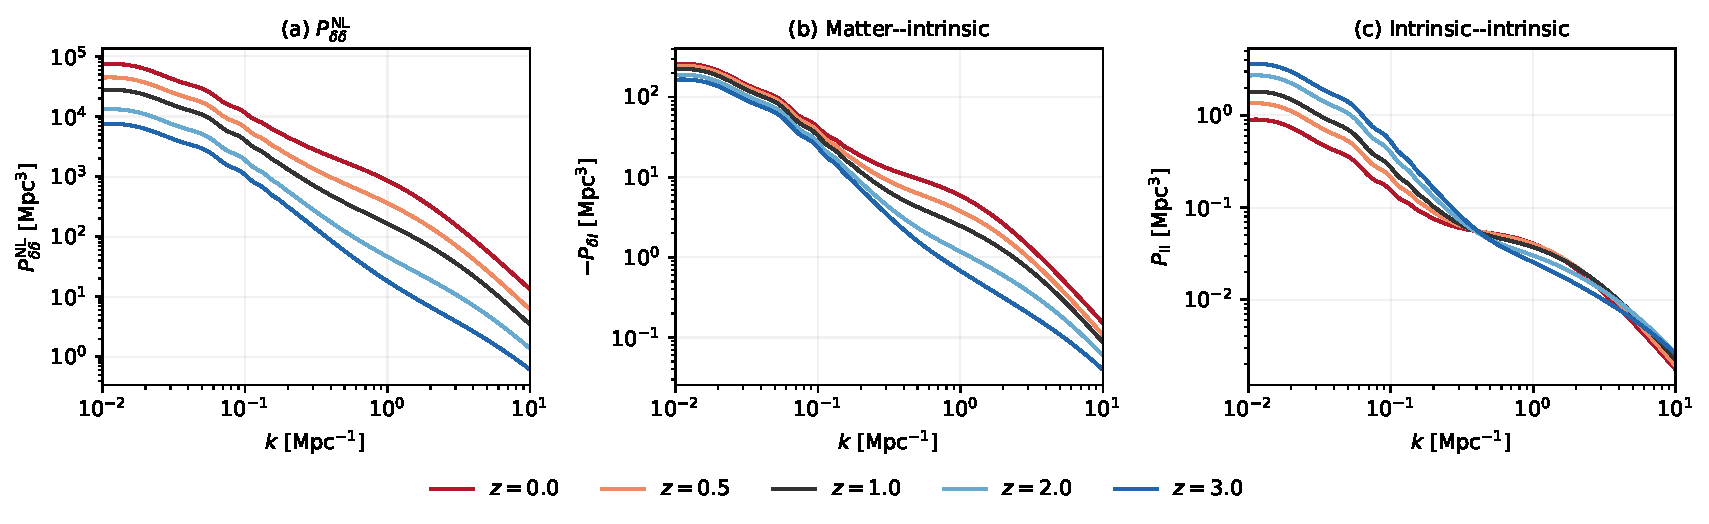
\includegraphics[width=\linewidth]{ia_power_spectra_panels.pdf}
  \caption{The three power spectra used in the NLA construction at five
  redshifts.  Panel (a) is the nonlinear matter spectrum.  Panel (b) shows
  $-P_{\delta I}$ because the adopted sign convention makes
  $P_{\delta I}<0$; the signed values, rather than their negatives, enter the
  model.  Panel (c) shows the positive $P_{II}$.  The same
  $\mathcal A_{\rm IA}$ enters linearly in panel (b) and quadratically in
  panel (c), which explains their different redshift ordering and amplitude.
  The curves use the notebook's Planck-like parameters and fiducial IA
  response, with an Eisenstein--Hu transfer function and Halofit nonlinear
  correction in PyCCL.  They illustrate the model relations and are not a
  fit to survey data.}
  \label{fig:ia-power-spectra}
\end{figure}

We factor the signed response as

\begin{equation}
  \mathcal A_{\rm IA}(k,z)
  = -A_0\,\mathcal A_\Omega(z)\,\mathcal A_\Theta(k,z).
  \label{eq:ia_decomposition}
\end{equation}

Here $A_0$ sets the overall IA strength.  The standard cosmological factor
$\mathcal A_\Omega(z)$ is proportional to $\Omega_{\rm m}/D(z)$, where
$D(z)$ is the linear growth factor.  The positive surface
$\mathcal A_\Theta(k,z)$ supplies the additional scale and redshift
flexibility tested in this project.  It is defined at the start because it is
the object later passed to PCA and the autoencoder:

\begin{equation}
  \mathcal A_\Theta(k,z)=R_z(z)R_L(z)S(k,z)>0.
  \label{eq:shape_surface}
\end{equation}

An overall multiplier is easy to compress and would say little about whether
a method had learned variation across the surface.  We therefore keep $A_0$
outside the 13-dimensional shape family and compress
$\log_{10}\mathcal A_\Theta$, not the signed full amplitude.  The three
factors in Equation~\ref{eq:shape_surface} have distinct roles: $R_z$
describes a broad redshift trend, $R_L$ adds a smooth transition, and $S$
describes scale dependence.

\subsection{The broad redshift factor \texorpdfstring{$R_z$}{Rz}}

Real lensing surveys contain galaxies observed at different cosmic times, so
an IA response that is fixed with redshift would be too narrow for this test.
We measure evolution relative to the fixed pivot $z_*=0.5$, which gives the
parameters a common reference point.  The factor $R_z$ is a power law in
$1+z$, controlled by $\eta$.  Its purpose is to represent a gradual increase
or decrease across the full redshift interval with one interpretable
parameter.  The exact definition is collected in
Appendix~\ref{app:detailed-equations}.

\subsection{The smooth transition factor \texorpdfstring{$R_L$}{RL}}

A single broad tilt cannot represent a response that changes behaviour around
an intermediate redshift.  The factor $R_L$ adds this second, smooth trend
without assigning an independent amplitude to every redshift bin.  The
parameter $\xi$ sets its strength and direction, $z_q$ locates the transition,
and $s$ controls how sharply it occurs.  The term ``luminosity-like'' describes
the shape of this phenomenological factor; it is not calibrated here to a
specific survey luminosity function.  Its definition is given in
Appendix~\ref{app:detailed-equations}.

\begin{figure}[!htbp]
  \centering
  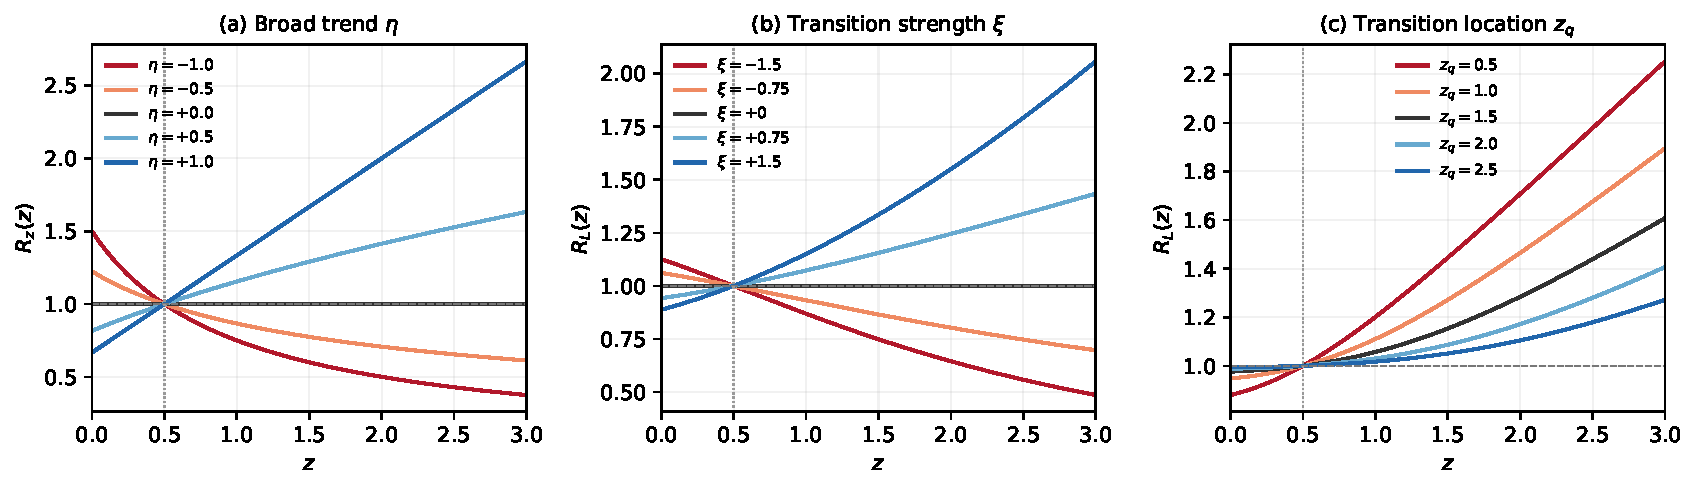
\includegraphics[width=0.86\linewidth]{ia_redshift_factors_panels.pdf}
  \caption{Redshift-factor parameters varied one at a time.  Panel (a) varies
  the broad trend $\eta$; panel (b) varies $\xi$ at fixed $s=2$ and
  $z_q=1.5$; panel (c) varies $z_q$ at fixed $\xi=1$ and $s=4$.  Every curve
  equals unity at the dotted pivot $z_*=0.5$.  These are phenomenological
  factors, not measured luminosity evolution.}
  \label{fig:ia-redshift-factors}
\end{figure}
\FloatBarrier

\subsection{The joint scale factor \texorpdfstring{$S(k,z)$}{S(k,z)}}

The factors $R_z$ and $R_L$ change only with redshift.  To represent the
additional uncertainty associated with nonlinear physical scales, we also
need a factor that changes across $k$.  Figure~\ref{fig:shape-surface} shows
the resulting two-dimensional $S(k,z)$ for the fiducial parameter choices.
Low $k$ corresponds to large physical scales and remains close to the
baseline $S=1$; the departure appears at higher $k$, where smaller physical
scales are being probed.  Its evolution across the vertical direction allows
the scale response itself to change with cosmic time.

\begin{figure}[!htbp]
  \centering
  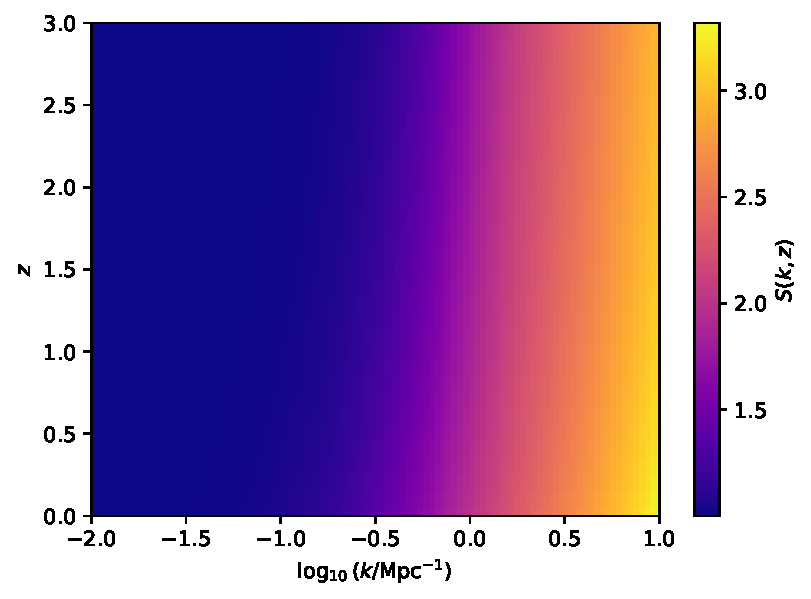
\includegraphics[width=0.72\linewidth]{ia_scale_redshift_surface.pdf}
  \caption{Fiducial scale--redshift factor $S(k,z)$.  The horizontal axis is
  $\log_{10}(k/{\rm Mpc}^{-1})$ and the vertical axis is redshift.  At
  $z_*=0.5$, the main choices are $k_{t,*}=0.5\,{\rm Mpc}^{-1}$, $q=1$,
  $n_*=2$, $\alpha=0.3$, and $m=2$.  The following subsections separate the
  role of each parameter and its redshift-evolution index.}
  \label{fig:shape-surface}
\end{figure}
\FloatBarrier

\subsection{The scale-correction strength \texorpdfstring{$q$}{q}}

The parameter $q$ controls the overall size of the scale-dependent
correction: $q=0$ removes that correction and returns $S=1$, while larger
sampled values make it more prominent.  Its operational physical meaning is
therefore the strength of the departure from the large-scale NLA baseline.
Varying $q$ is needed to test whether compression works for both nearly
scale-independent and strongly scale-dependent surfaces.  It does not claim
that the strength of real small-scale IA is known.

\subsection{The transition scale \texorpdfstring{$k_t(z)$}{kt(z)}}

The correction should not affect all wavenumbers equally.  Large scales are
closer to the regime in which the NLA prescription is normally used, whereas
additional uncertainty is expected as $k$ increases.  We therefore use
$k_t(z)$ to mark where the scale correction begins to turn on:
$k\ll k_t$ is close to the large-scale baseline, and $k\gtrsim k_t$ is
increasingly affected by $S$.  The particular smooth transition used here is
a construction of this project, not a new physical law or an observationally
measured boundary.  Its purpose is to represent uncertainty in the onset of
small-scale behaviour, not to solve the underlying small-scale physics.
$k_{t,*}$ fixes the transition at $z_*=0.5$, and $\gamma_t$ allows that
location to move with redshift.

\subsection{The transition sharpness \texorpdfstring{$n(z)$}{n(z)}}

Knowing the location of a transition is not enough: the response may change
gradually across a broad range of scales or relatively rapidly near $k_t$.
The factor controlled by $n(z)$ distinguishes these possibilities.  Smaller
$n$ gives a broader turn-on and larger $n$ gives a sharper one.  Introducing
this freedom avoids imposing one arbitrary transition width on every
synthetic surface.  The pivot value $n_*$ sets the sharpness at $z_*=0.5$,
while $\gamma_n$ allows the width of the transition to evolve.

\subsection{The high-\texorpdfstring{$k$}{k} slope
\texorpdfstring{$\alpha(z)$}{alpha(z)}}

After the correction has turned on, its amplitude need not approach a flat
plateau.  The parameter $\alpha(z)$ therefore controls the asymptotic
high-$k$ trend: positive values allow the response to continue increasing,
negative values allow it to decrease, and $\alpha=0$ gives no additional
high-$k$ tilt.  This factor is included because a compression method should
not succeed only when every small-scale tail has the same slope.  The pivot
value $\alpha$ specifies the slope at $z_*=0.5$, and $\gamma_\alpha$ controls
its redshift evolution.

\subsection{The tail smoothness \texorpdfstring{$m(z)$}{m(z)}}

The high-$k$ slope must join the transition without an unphysical corner.
The parameter $m(z)$ controls how smoothly the model bends toward its
asymptotic tail.  It is kept separate from $n(z)$ because $n$ controls how the
scale correction switches on, whereas $m$ controls the curvature of the tail
after that onset.  This distinction lets the dataset contain surfaces with
similar transition locations but different detailed shapes.  The pivot value
$m$ and evolution index $\gamma_m$ set this behaviour across redshift.  The
complete expression combining $q$, $k_t$, $n$, $\alpha$, and $m$ is given in
Appendix~\ref{app:detailed-equations}.

These quantities are phenomenological shape controls rather than direct
observables.  The pivot parameters specify the scale response at $z_*$, and
the four dimensionless $\gamma$ indices specify how those controls evolve
away from the pivot.  Their physical interpretation is therefore
operational---strength, onset scale, transition width, tail slope, and tail
curvature---rather than a claim that each parameter corresponds to one
independently measurable galaxy property.

\subsection{Sampling and checking the 13-parameter model family}

The 13 parameters comprise four redshift and transition parameters, five
pivot-scale shape parameters, and four parameters controlling redshift
evolution.  A large ensemble is needed because PCA and a neural network should
be tested on the family as a whole, not on a few hand-picked curves.  We draw
100,000 combinations from documented data-generation
bounds; the complete ranges and sampling distributions are listed in
Appendix Table~\ref{tab:sampling-bounds}.  Each combination produces a
surface on 31 redshift points from $z=0$ to $z=3$ and 101 logarithmically
spaced wavenumbers from $k=0.01$ to $10\,\mathrm{Mpc}^{-1}$.  The redshift
grid covers the survey-relevant evolution represented by the model, while
logarithmic spacing resolves changes across several decades in scale.

Random samples alone can miss failures at the edges of a high-dimensional
box.  Before fixing these bounds, we therefore evaluated
8,192 random draws and all $2^{13}=8{,}192$ corners of the parameter box.  All
of those surfaces were finite and positive.  Dynamic-range checks were used
to keep the family broad enough for compression tests without allowing
unmanageably extreme corner cases.

\reportfigure{sampling_amplitude_ensemble.pdf}{Distribution of 8,192 random
sampling-range validation surfaces at $z=0$ and $z=3$.  The shaded regions contain the
central 98\% and 90\% of $\mathcal A_\Theta$ at each $k$, the black curve is
the median, and the colored curves are the five surfaces with the largest
internal dynamic range.  All evaluated surfaces are finite and strictly
positive.}{fig:sampling-ensemble}

\subsection{Training, validation, and test subsets}

Evaluating a model on the same surfaces used to fit it would overstate how
well it generalizes.  The stored split therefore contains 80,000 training
surfaces, 10,000 validation surfaces, and 10,000 test surfaces.  The training
subset fits the PCA basis and autoencoder; the validation subset supports
model selection and diagnostics; and the test subset remains unused until
all choices have been frozen.  Normalization statistics and the PCA basis are
calculated from training data only so that information from held-out surfaces
cannot influence the fitted representations.

This is a phenomenological model family.  The sampled ranges are documented
data-generation bounds, not observational constraints, and the surfaces have
not been calibrated to a particular galaxy survey.  The resulting dataset
therefore gives us a controlled test of compression: every surface has the
same $(k,z)$ grid, but the underlying parameters vary across the prescribed
13-dimensional space.  In the next section, we use this dataset to test
whether the $3{,}131$ grid values can be represented by a much smaller latent
vector.

\clearpage

\section{Compressing the surfaces with an autoencoder}
\label{sec:autoencoder}

Section~\ref{sec:model} constructed the surface dataset.  Here we transform and
normalize each surface before passing it through three one-dimensional
convolutional layers and a two-number bottleneck.  The decoder reconstructs the
full grid from those two values.  The purpose is not merely to build a neural
network: it is to test whether a nonlinear map can preserve more information
than PCA when both methods are restricted to the same two-number
representation.  Section~\ref{sec:results} makes that matched comparison.

\subsection{Input transformation and normalization}

Large amplitudes would dominate an error measured directly on the positive
surface, even when a smaller-amplitude region has an equally important
fractional error.  The encoder therefore receives the pointwise log-surface
$Y=\log_{10}\mathcal A_\Theta$, which turns multiplicative differences into
additive ones.  We then subtract the mean
training surface $\overline{Y}$ and divide by its global root-mean-square
deviation $\sigma$.  Both quantities are computed from the training split and
then applied unchanged to validation and test data.  Using one global scale,
rather than a different scale at each $(k,z)$, keeps the relative size of
features across the grid and avoids leakage from the held-out subsets.  The
full transformation is recorded in Appendix~\ref{app:detailed-equations}.

\subsection{From 3,131 values to a two-number bottleneck}

The bottleneck is the part that tests the project's compression question.
An autoencoder contains an \emph{encoder} and a \emph{decoder}.  The encoder
maps a surface $\bm{x}$ to a latent vector $\bm{z}$, and the decoder maps
$\bm{z}$ to a reconstruction $\widehat{\bm{x}}$.  We set
$\bm{z}\in\mathbb{R}^{2}$ to match the two-component PCA baseline and to make
this pilot representation easy to inspect.  Because no skip connection
bypasses the bottleneck, every reconstructed surface must genuinely pass
through two numbers.  Otherwise good reconstruction could come from a hidden
high-dimensional route rather than compression.  The compact mathematical
definition is included in Appendix~\ref{app:detailed-equations}.

One-dimensional convolutions first collect nearby structure along wavenumber.
Dense layers then summarize the whole surface.  The bottleneck keeps only two
coordinates, from which the decoder must rebuild the full grid.  Successful
reconstruction would therefore indicate that the sampled surfaces lie near a
lower-dimensional nonlinear structure; failure would show that two
coordinates discard too much information.

\subsection{Why use one-dimensional convolutions?}

Neighboring wavenumbers are strongly related because the analytic response
changes smoothly and contains scale transitions.  We therefore arrange the
input as 31 redshift channels, each containing a 101-point sequence in
wavenumber.  A one-dimensional convolution slides along that sequence and
learns local scale-dependent patterns.  Reusing the same kernel at different
$k$ positions lets the network recognize similar transitions without learning
a separate weight for every grid cell, while its filters mix information
between redshift channels.  This is a motivated first architecture, not a
claim that Conv1D is uniquely optimal; its advantage must be judged against
the held-out reconstruction results.

\subsection{Network architecture}

\begin{table}[t]
\centering
\caption{Configured three-layer Conv1D autoencoder with latent dimension 2.
Sequence lengths refer to the
wavenumber axis.}
\label{tab:architecture}
\begin{tabular}{@{}lll@{}}
\toprule
Stage & Shape or width & Main operation \\
\midrule
Input & $31\times101$ & normalized $\log_{10}\mathcal A_\Theta$ \\
Encoder 1 & $64\times51$ & Conv1D, kernel 5, stride 2, SiLU \\
Encoder 2 & $128\times26$ & Conv1D, kernel 5, stride 2, SiLU \\
Encoder 3 & $256\times13$ & Conv1D, kernel 3, stride 2, SiLU \\
Flatten & $3{,}328$ & flatten $256\times13$ features \\
Dense encoder & $3{,}328\rightarrow256\rightarrow64$ & nonlinear summary \\
Bottleneck & $2$ & latent coordinates \\
Dense decoder & $2\rightarrow64\rightarrow256\rightarrow3{,}328$ & expand latent representation \\
Decoder & reverse sequence & transposed convolutions \\
Output & $31\times101$ & reconstructed normalized surface \\
\bottomrule
\end{tabular}
\end{table}

The encoder gradually shortens the wavenumber sequence while increasing the
number of learned features; the decoder reverses this process.  This gives the
network enough capacity to test a nonlinear representation without relaxing
the two-number information bottleneck.  The resulting model has 2,039,969
trainable weights.  That large weight count should not be confused with the
latent dimension: the project tests compact representation of each surface,
not a network with only two trainable parameters.  We use SiLU activations and
no skip connections; a skip connection would let information avoid the
bottleneck and invalidate the comparison with two-component PCA.

\subsection{Training objective and model selection}

The training target should reward accurate reconstruction over the whole
surface rather than at one selected scale.  We therefore minimize mean squared
error in normalized log-amplitude space, averaged over every sample, redshift,
and wavenumber value in a batch.  Its explicit definition is given in
Appendix~\ref{app:detailed-equations}.  Table~\ref{tab:training-config}
shows only the choices needed to understand the training logic; complete
numerical settings are listed in Appendix
Table~\ref{tab:training-config-details}.
These settings describe the current shared template.  The preliminary
autoencoder metrics in Section~\ref{sec:results} come from a separate
25-epoch run, not from a completed run of this longer schedule; the table must
not be read as the provenance of those reported numbers.

\begin{table}[htbp]
\centering
\small
\caption{Main choices in the shared autoencoder training template.}
\label{tab:training-config}
\begin{tabularx}{\linewidth}{@{}
  >{\raggedright\arraybackslash}p{0.19\linewidth}
  >{\raggedright\arraybackslash}p{0.25\linewidth}
  >{\raggedright\arraybackslash}X@{}}
\toprule
Setting & Configured value & Purpose \\
\midrule
Objective & MSE in normalized $\log_{10}\mathcal A_\Theta$
  & Reconstruct the full surface while treating multiplicative amplitude
    differences more evenly. \\
Optimizer & AdamW, learning rate $2\times10^{-4}$
  & Learn nonlinear weights with adaptive updates. \\
Batch size & 512 surfaces
  & Balance stable updates with memory use. \\
Training control & Reduce the learning rate after a plateau; stop early
  & Refine stalled optimization without training indefinitely. \\
Model selection & Lowest validation MSE
  & Select performance on unseen surfaces rather than training fit. \\
Success benchmark & Recovered variance $\geq 99.9\%$
  & Set a demanding compression goal, not a cosmological requirement. \\
\bottomrule
\end{tabularx}
\end{table}
\clearpage

\subsection{What must be checked beyond the average loss?}

An average MSE can look good even if the model fails badly for a small region
or a difficult surface.  Such a failure matters because a localized IA error
could propagate differently into a lensing analysis.  We therefore use
several complementary diagnostics:

\begin{description}
  \item[Log-space RMSE] measures the typical reconstruction residual
  $\widehat Y-Y$ in dex over all validation grid values.  It is closely tied
  to the training objective, but its logarithmic units are not an immediate
  fractional error in physical amplitude.

  \item[Recovered variance] is one minus the reconstruction sum of squares
  divided by the validation set's total squared distance from the training
  mean.  It answers how much of the surface-to-surface variation survives
  compression and permits a direct comparison with PCA.  A high value can
  still conceal a localized failure.

  \item[Mean physical relative error] converts each log residual back to
  amplitude space using
  $\lvert 10^{(\widehat Y-Y)}-1\rvert$ and averages over surfaces and grid
  cells.  This quantity is easier to interpret fractionally, but positive and
  negative log residuals produce asymmetric amplitude errors.

  \item[Per-surface relative RMSE] first summarizes the physical relative
  errors across all 3,131 cells of each surface.  Its 95th percentile then
  describes a difficult but not single worst-case part of the validation
  population.  This prevents a small set of poorly reconstructed surfaces
  from disappearing inside a global mean.
\end{description}

Error maps over $(k,z)$ and parameter space are also needed to locate where a
model fails, while maximum-error summaries can flag isolated extreme cells.
The preliminary run available for this report provides only the scalar
summaries reported in Section~\ref{sec:results}; its checkpoint is unavailable
for generating new maps.  Finally, the $99.9\%$ recovered-variance target is
an internal compression benchmark, not evidence that reconstruction errors
are already small enough for cosmology.  That requires propagating them into
lensing observables and parameter inference.

\section{Results and discussion}
\label{sec:results}

All autoencoder numbers in this section are validation results.  The test
split has not been read.

\subsection{PCA: the linear compression baseline}

PCA finds orthogonal linear patterns that account for the largest variation in
the training surfaces.  Each surface is flattened from
$31\times101$ to 3,131 values, centered using the training mean, and projected
onto the leading patterns.  The first two PCA components retain about 96.23\%
of validation variance.  On the same validation split, ten components recover
about 99.94\% of the variance.  Separately, the rank-25 PCA fit accounts for
99.9986\% of training variance.

Figure~\ref{fig:pca-variance} shows the individual and cumulative training
variance, while Figure~\ref{fig:pca-rank} shows validation reconstruction
error as the rank increases.  Most of the gain appears in the first few
components.

\reportfigure{pca_explained_variance.pdf}{Individual and cumulative variance
explained by PCA fitted to the training surfaces.  Table~\ref{tab:preliminary-results}
instead reports reconstruction on the validation set.}{fig:pca-variance}

\reportfigure{pca_reconstruction_error_by_rank.pdf}{Validation reconstruction
error as the number of PCA components increases.  Rank 2 is the matched
baseline for the autoencoder; rank 10 is shown as a higher-dimensional
reference.}{fig:pca-rank}

\subsection{Autoencoder result with a two-number latent representation}

The autoencoder measurements currently available come from an earlier
25-epoch trial, not from the longer training configuration described in
Section~\ref{sec:autoencoder}.  Its best checkpoint, at epoch 20, recovers
98.09\% of the validation variance with a two-number latent space.  The
validation RMSE is 0.03795 in $\log_{10}\mathcal A_\Theta$, the mean relative
error in physical amplitude is 6.48\%, and the 95th percentile of per-surface
relative RMSE is 13.95\%.  Only the scalar summaries from that trial are
available in this report; its checkpoint and training history are not present
in the current repository.  The comparison is therefore preliminary.

\subsection{A fair comparison at equal latent dimension}

Table~\ref{tab:preliminary-results} compares methods on the same validation
indices and the same log-amplitude target.  The main comparison is autoencoder
dimension 2 versus PCA rank 2.  PCA rank 10 is included only as a
higher-dimensional accuracy reference.

\begin{table}[t]
\centering
\caption{Preliminary validation comparison on the stored 10,000-surface
validation
split.  The autoencoder uses a two-number bottleneck.  PCA rank 2 is the
matched-dimension baseline.  PCA rank 10 is a higher-dimensional reference,
not a competing two-number method.}
\label{tab:preliminary-results}
\begin{tabular}{@{}lrrrr@{}}
\toprule
Method & Latent size & Variance recovered & Log RMSE & Mean relative error \\
\midrule
PCA & 2 & 0.9623 & 0.0533 & 0.0866 \\
Conv1D autoencoder & 2 & 0.9809 & 0.0380 & 0.0648 \\
PCA & 10 & 0.9994 & 0.0068 & 0.0104 \\
\bottomrule
\end{tabular}
\end{table}

In this trial, the autoencoder has higher recovered variance and lower
reconstruction errors than PCA at the same latent dimension.  This suggests
that two linear components do not capture the model family as efficiently as
the nonlinear mapping.  It does not show that two numbers are sufficient:
the 99.9\% variance target was not reached, and the 95th-percentile result
shows that some surfaces are substantially harder to reconstruct.

\subsection{Latent-space interpretation}

We have not yet mapped the two latent coordinates against the 13 input
parameters, so neither coordinate is given a physical interpretation.  Such an
analysis should examine both parameter correlations and reconstructed surfaces
along paths through the latent space.

\subsection{Limitations}

These results have four main limitations:

\begin{itemize}
  \item The analytic response is a deliberately flexible, phenomenological
        model family.  It has not yet been calibrated to a particular survey or
        shown to describe all physical intrinsic-alignment effects.
  \item The autoencoder numbers above come from validation data.  The untouched
        test split will be evaluated only after the architecture and latent
        dimension have been chosen.
  \item The autoencoder result comes from one short run whose checkpoint and
        training history are unavailable; it has not been repeated across
        several random seeds.
  \item Reconstruction accuracy varies across surfaces, so the mean metrics do
        not establish adequate precision at every scale, redshift, or
        parameter-space location.
\end{itemize}

\subsection{Next steps}

\begin{enumerate}
  \item compare latent dimensions 2, 4, 6, 8,
        and 10, using the same data and metrics;
  \item repeat the most promising model with several random seeds;
  \item map reconstruction error over $(k,z)$ and over the 13-parameter space;
  \item test whether a physically motivated weighted loss improves important
        regions without worsening the rest of the surface; and
  \item after selecting the method, evaluate the untouched test set.
\end{enumerate}

\section{Summary and Future Prospects}
\label{sec:summary}

Section~\ref{sec:results} compared the Conv1D autoencoder with PCA and showed
both the promise and the current limitations of two-number compression.  This
section summarizes the main conclusions and the next steps of the project.

To isolate compression from observational uncertainty, the comparison uses
100,000 controlled surfaces generated by varying 13 sampled shape parameters.
Each surface contains 3,131 values over redshift and wavenumber.  PCA provides
the linear baseline, while the Conv1D autoencoder forces the same surface
through a two-number bottleneck.  Holding the representation length fixed is
what lets the experiment test the value of nonlinearity rather than the value
of storing more numbers.

On the held-out validation set, the autoencoder with a two-number latent space
recovers $98.09\%$ of the total variance, compared with $96.23\%$ for
two-component PCA.  At the same latent dimension, the nonlinear autoencoder
therefore reconstructs the surfaces more accurately than the linear PCA
baseline.  This suggests that the model family contains structure that is not
captured as efficiently by two linear PCA components.  However, these
measurements come from a preliminary short run.  The autoencoder has not met
the $99.9\%$ recovered-variance target or been evaluated on the test set, and
its errors remain sizeable for difficult surfaces.  The result therefore
supports continuing the nonlinear approach, but not yet replacing the
13-parameter description in a cosmological analysis.

The next step is to test larger latent dimensions, which will show how much
accuracy is gained by relaxing the two-number constraint, and to repeat the
most promising configurations with several random seeds, which will test
whether the gain is reproducible.  Once the architecture and latent dimension
have been chosen, the untouched test set can provide the final generalization
check.  In the longer term, the model family should be connected more directly
to physical intrinsic-alignment calculations and survey requirements, because
surface reconstruction is useful only if its errors are small where they
matter for lensing inference.


\clearpage
\section*{Acknowledgements and contributions}
\addcontentsline{toc}{section}{Acknowledgements and contributions}

\draftnote{The current competition instructions require this material to be
detailed and truthful.  Expand it to the required 1--2 pages (500--1,500 words)
and check the instructions for the student’s regional competition before
submission.  Do not submit the prompts below as if they were completed prose.}

\subsection*{Research background and supervision}

\placeholder{Explain how the topic was chosen, how the student and supervisor
began working together, what form the supervision took, and whether the
supervision was paid.  Identify any university, institute, laboratory, or other
person who provided assistance, access, code, data, or computing resources.}

\subsection*{Division of work}

\begin{longtable}{@{}>{\raggedright\arraybackslash}p{0.23\linewidth}
  >{\raggedright\arraybackslash}p{0.31\linewidth}
  >{\raggedright\arraybackslash}p{0.37\linewidth}@{}}
\toprule
Stage & Student contribution & Supervisor or external contribution \\
\midrule
Topic and research question & \placeholder{specific work} & \placeholder{specific guidance} \\
Background reading & \placeholder{sources read and summarized} & \placeholder{reading suggestions} \\
Analytic model & \placeholder{derivation, implementation, checks} & \placeholder{guidance or review} \\
Dataset generation & \placeholder{sampling and validation work} & \placeholder{guidance or resources} \\
PCA analysis & \placeholder{implementation and interpretation} & \placeholder{guidance or review} \\
Autoencoder & \placeholder{design, code, training, diagnostics} & \placeholder{guidance or review} \\
Figures and tables & \placeholder{figures created and checked} & \placeholder{feedback} \\
Report writing & \placeholder{sections written and revised} & \placeholder{comments and language help} \\
\bottomrule
\end{longtable}

\subsection*{Difficulties and how they were solved}

\placeholder{Describe concrete difficulties encountered during the project,
how the student investigated them, which attempts failed, what evidence changed
the approach, and what the student learned.}


\clearpage
\phantomsection
\addcontentsline{toc}{section}{References}
\begin{thebibliography}{99}
\small
\setlength{\bibsep}{0.6em}
\input{Reference.bib}
\end{thebibliography}

\end{document}
